% ICASSP 2027 submission — "When to Steer"
% Build: latexmk -pdf main.tex   (needs spconf.sty + IEEEbib.bst from the ICASSP 2027 paper kit)
\documentclass{article}
\usepackage{spconf,amsmath,amssymb,graphicx,booktabs,multirow,xcolor,url}
\usepackage[hidelinks,pdftitle={When to Steer: Sensitivity-Calibrated Probe Guidance for Controllable Music Diffusion},pdfauthor={Yushi Ye, Wilson Zheng, Yongyi Zang}]{hyperref}
\urlstyle{same}
% auto-generated by make_figures.py
\newcommand{\cohMLSP}{0.363}
\newcommand{\cohRAPG}{0.445}
\newcommand{\cohSAO}{0.126}
\newcommand{\corrRF}{0.96}
\newcommand{\peakDC}{54\%}
\newcommand{\peakF}{88\%}
\newcommand{\dRvsMid}{+0.022}
\newcommand{\pRvsMid}{p<10^{-6}}
\newcommand{\winsRvsMid}{129 of 195}
\newcommand{\dRvsTopK}{+0.011}
\newcommand{\pRvsTopK}{p<10^{-5}}
\newcommand{\winsRvsTopK}{122 of 184}
\newcommand{\dTopKvsMid}{+0.010}
\newcommand{\pTopKvsMid}{p=0.002}
\newcommand{\winsTopKvsMid}{115 of 193}
\newcommand{\pTopKvsMLSP}{p<10^{-6}}
\newcommand{\placementShare}{86\%}
\newcommand{\cohTopK}{0.434}
\newcommand{\cohMid}{0.424}
\newcommand{\lamRealised}{0.057}
\newcommand{\cohGainAbs}{0.32}
\newcommand{\rhoFixedT}{0.27}
\newcommand{\rhoFixedTlate}{0.57}
\newcommand{\rhoFixedTpos}{86\%}
\newcommand{\looRange}{26--30}
\newcommand{\looRangeS}{0.54--0.62}
\newcommand{\bootPeakShare}{92\%}
\newcommand{\sigmaAtEighteen}{27}
\newcommand{\tAtEighteen}{0.96}
\newcommand{\sigmaAtThirtyTwo}{3.2}
\newcommand{\tAtThirtyTwo}{0.76}
\newcommand{\sigmaAtPeak}{8.0}
\newcommand{\tAtPeak}{0.89}
\newcommand{\sigmaAtFourteen}{49}
\newcommand{\tAtFourteen}{0.98}
   % auto-generated from results/ by w2s/scripts/make_figures.py
% auto-generated by make_figures.py (Exp D)
\newcommand{\budgetKs}{5,10,15,25}
\newcommand{\cohUniKv}{0.16}
\newcommand{\cohTopKv}{0.26}
\newcommand{\cohUniKx}{0.24}
\newcommand{\cohTopKx}{0.38}
\newcommand{\cohUniKxv}{0.30}
\newcommand{\cohTopKxv}{0.48}
\newcommand{\cohUniKxxv}{0.40}
\newcommand{\cohTopKxxv}{0.56}
\newcommand{\budgetUniMax}{0.40}
\newcommand{\budgetUniMaxK}{25}
\newcommand{\budgetTopMatchK}{15}

% auto-generated by make_figures.py (SA3 transfer)
\newcommand{\saThreePeakF}{76\%}
\newcommand{\saThreePeakDC}{22\%}
\newcommand{\saThreeCorrRF}{0.93}
\newcommand{\saThreeDCpeak}{0.089}
\newcommand{\saThreeDCearly}{0.079}
\newcommand{\saThreeDClate}{0.017}
\newcommand{\saThreeFmax}{0.31}
\newcommand{\saThreeTpeak}{0.99}
\newcommand{\saThreeCohSAO}{0.09}
\newcommand{\saThreeCohEarly}{0.44}
\newcommand{\saThreeCohMid}{0.40}
\newcommand{\saThreeCohLate}{0.18}
\newcommand{\saThreeCohUni}{0.43}
\newcommand{\saThreeCohMLSP}{0.28}
\newcommand{\saThreeCohRAPG}{0.47}
\newcommand{\saThreeCohTopK}{0.44}
\newcommand{\saThreePRAPGvsMLSP}{10^{-4}}
\newcommand{\saThreeRAPGsteps}{4--18}


\def\x{{\mathbf x}}
\def\z{{\mathbf z}}
\def\y{{\mathbf y}}
\def\g{{\mathbf g}}
\newcommand{\TODO}[1]{\textcolor{red}{[#1]}}
\newcommand{\rms}{\operatorname{rms}}
\newcommand{\AFFZANG}{Independent Researcher}   % as on arXiv:2609.04516 (MLSP 2026 paper); confirm with the author before submission
\newcommand{\LEGACYNOTE}{ (with the original placement the same schedule scores $0.259$ against the true melody and $0.68$ against its first pitch class alone, so the finding of~\cite{ye2026pitchclass} that guidance raises coherence stands, but its outputs followed the first note)}
\newcommand{\RANDNOTE}{ A control burst in a random direction of identical update norm, applied at the peak position, changes coherence by $0.003$ (n.s.) against $0.104$ for the probe gradient (paired $p{<}10^{-6}$), so the effect is directed rather than a by-product of perturbing a noisy latent.}
\newcommand{\EARLYNOTE}{ The early window is inert only at this step size. With $\lambda{=}\alpha{=}0.2$, $0.5$ and $1.0$ its development-set coherence rises from $0.12$ (unguided) to $0.23$, $0.29$ and $0.41$ while CLAP falls from $0.207$ to $0.187$, $0.184$ and $0.173$, so a method that pushes hard early, as LatCH may, can steer there at a quality cost; at matched update norm the mid window is where a step counts most.}
\newcommand{\RANDNOTESAThree}{ The random-direction control at the same norm gives $-0.026$ against $0.089$ for the probe gradient (paired $p{<}10^{-4}$).}
\newcommand{\LAMROBUST}{ Repeating the sweep at the $\lambda{=}0.05$ of the main experiments gives the same profile (peak at $s{=}0.54$, $\Delta C{=}0.099$ vs $0.104$, Pearson $0.99$ between the curves; the top-15 steps shift by one, to 18--32).}

\title{When to Steer: Sensitivity-Calibrated Probe Guidance\\for Controllable Music Diffusion}
\name{Yushi Ye$^{\star\dagger}$ \qquad Wilson Zheng$^{\star\dagger}$ \qquad Yongyi Zang$^{\star\ddagger}$\thanks{$^{\star}$Equal contribution.}}
\address{$^{\dagger}$Carnegie Mellon University, Pittsburgh, PA, USA \qquad $^{\ddagger}$\AFFZANG\\\{yushiye, wilsonz\}@andrew.cmu.edu, zyy0116@gmail.com}

\begin{document}
\ninept
\maketitle
% For camera-ready, uncomment the IEEE copyright notice (see ICASSP 2027 paper kit):
% \copyrightnotice{\copyright\ 2027 IEEE. Personal use of this material is permitted. Permission from IEEE must be obtained for all other uses.}

\begin{abstract}
Latent-space probes give cheap gradients for steering diffusion-based music generation, but existing methods apply the guidance on hand-picked subsets of sampling steps: on Stable Audio Open, recent work intervenes either only in the first 20\% of denoising or only in the last 60\%, and neither choice was measured. We ask \emph{when} probe guidance should be applied. Along real Stable Audio Open trajectories we measure how the pitch-class decodability of a 125k-parameter probe evolves and, by intervening at single positions, where a guidance step actually changes the output. The two peak at different stages: decodability keeps rising until denoising is nearly complete (\peakF), whereas a guidance step changes the output most around the middle of sampling (\peakDC), so where the probe is most accurate is not where it steers best. Spending a fixed budget of updates at the steps of highest measured steering sensitivity raises melodic coherence from \cohMLSP\ (the fixed window of prior work) to \cohTopK\ at matched compute, with prompt adherence (CLAP) and audio realism (Fr\'echet distance) unchanged; scaling each step by a target-free reliability signal adds a small further gain (\cohRAPG), and a reliability threshold, which follows decodability, adds none. On Stable Audio 3 the sensitive window lies at the start of its trajectory rather than mid-way, again far from where the probe is most reliable: the window is model-specific, but one burst sweep on a handful of development prompts locates it in either model.
\end{abstract}

\begin{keywords}
controllable music generation, latent diffusion, training-free guidance, probing, guidance scheduling
\end{keywords}

\section{Introduction}
\label{sec:intro}
Text-to-music diffusion models such as Stable Audio Open~\cite{evans2024stableaudioopen} (SAO) produce high-quality audio but give the user only coarse control through the text prompt. Trained conditioning offers melody control~\cite{wu2024musiccontrolnet,copet2023musicgen}. Inference-time guidance adds it without retraining, by evaluating a differentiable target loss on the partially denoised sample and using its gradient to nudge the latent~\cite{dhariwal2021diffusion,bansal2023universal,yu2023freedom,ye2024tfg,levy2023controllable}, or by optimising the sampler through its own trajectory~\cite{novack2024ditto}. For music transformers, probe-steered activations with a self-monitoring signal~\cite{koo2024smitin} are the closest relative of the reliability signal used here. For latent audio diffusion, back-propagating through the audio decoder is expensive, so two recent works replace the decoder-plus-feature-extractor by a small network that reads the control directly from the latent: latent-control heads (LatCH)~\cite{novack2026latch} and pitch-class probes~\cite{ye2026pitchclass}. Both operate on SAO, both are cheap, and both use a fixed schedule chosen by hand.

Curiously, the two schedules are opposite. LatCH applies its ``selective'' guidance only during the first 20\% of steps, arguing that later interventions drift off the data manifold~\cite{novack2026latch}, whereas~\cite{ye2026pitchclass} waits until 40\% of denoising is complete and then intervenes every second step, arguing that early latents are too noisy for the probe. Neither work reports an ablation of the interval, and the heads of~\cite{novack2026latch} include a monophonic pitch head, so its window was chosen for pitch control as well. The question is not specific to these two methods. Limited-interval guidance is known to matter for classifier-free guidance in image diffusion~\cite{kynkaanniemi2024interval}, and training-free guidance frameworks expose the interval as a hyper-parameter~\cite{ye2024tfg}. For probe-based latent guidance of music there is no principled answer, and the answer is not obvious, because the probe's information content, the effect of a gradient step and its cost in audio quality all change along the trajectory, and not necessarily together.

This paper studies that question on SAO with the pitch-class probe of~\cite{ye2026pitchclass}, and turns the answer into a schedule calibrated by measurement. Our prior work showed that a lightweight latent probe can steer pitch-class content, and here we ask when it should. Our contributions are:
\begin{enumerate}\setlength\itemsep{0pt}
\item \textbf{Trajectory-wise reliability analysis.} We record real SAO trajectories and score the probe at every step against labels transcribed from the generated audio. Decodability reaches 95\% of its maximum only at \peakF\ of the trajectory, and the target-free reliability $R_t$ of the probe tracks it (Pearson \corrRF).
\item \textbf{Steerability $\neq$ decodability.} Decodability describes what can be read from a latent. To find where a guidance step actually changes the output, we intervene at single positions of the trajectory. Steering sensitivity peaks near the middle of sampling (\peakDC), far earlier than decodability saturates, and a burst of updates there changes melodic coherence several times more than the same burst applied late, where the probe is far more accurate. With the update rule of~\cite{ye2026pitchclass}, the early window of prior selective guidance barely moves pitch-class content on SAO, yet it is close to optimal on Stable Audio 3 (Sec.~\ref{sec:sa3}), so the window has to be measured for each model.
\item \textbf{Sensitivity-calibrated probe guidance (SCPG).} A schedule that spends a fixed budget of $K$ updates on the $K$ steps of highest measured steering sensitivity. It matches or improves on every fixed window we tested and locates the best of them without a window sweep. Scaling the step by the probe's reliability adds a small further gain, and an online reliability threshold, which follows decodability, does not help.
\end{enumerate}
We also correct the target/latent alignment of the public implementation of~\cite{ye2026pitchclass} (Sec.~\ref{sec:setup}); all numbers use the corrected code. Code, per-run results and audio examples are online.\footnote{\url{https://stoneyey.github.io/mic-pitch-class-steering/}}

\section{Method}
\label{sec:method}

\subsection{Probe-guided sampling}
SAO~\cite{evans2024stableaudioopen} denoises a latent $\z\in\mathbb{R}^{64\times T}$ ($T{=}1024$ frames at 21.5\,Hz) with a diffusion transformer and an EDM-style sampler~\cite{karras2022edm}; we use $N{=}50$ steps and classifier-free guidance~\cite{ho2022cfg} of 4.0. Step $t$ denotes the latent returned by the $t$-th scheduler update, to which guidance is applied before the next denoising step; positions are reported as denoising progress $s{=}t/N\in[0,1]$. A convolutional probe $f_\phi$ with 125k parameters, trained on VAE latents of MAESTRO~\cite{hawthorne2019maestro} with Gaussian-noise augmentation, maps a latent to frame-level pitch-class probabilities $p_t{=}f_\phi(\z_t)\in[0,1]^{12\times T}$~\cite{ye2026pitchclass}. Given a target pitch-class roll $\y^\star\in\{0,1\}^{12\times T}$, the guidance loss is the binary cross-entropy $\mathcal{L}_t{=}\mathrm{BCE}(p_t,\y^\star)$ restricted to the audible frames, with gradient $\g_t{=}\nabla_{\z_t}\mathcal{L}_t$, and the latent is updated with the RMS-normalised, clamped step of~\cite{ye2026pitchclass}:
\begin{equation}
\z_t \leftarrow \z_t - \operatorname{clamp}\!\Big(\lambda_t\,\tfrac{\rms(\z_t)}{\rms(\g_t)}\,\g_t,\ \pm\alpha\,\rms(\z_t)\Big),
\label{eq:update}
\end{equation}
with $\alpha{=}0.05$. In~\cite{ye2026pitchclass}, $\lambda_t{=}\lambda$ is constant and the update fires on a hand-chosen set of steps $\mathcal{T}$ (every second step after 40\% of denoising, i.e.\ $K{=}15$ updates); in LatCH the set is the first 20\% of steps. Everything that follows changes only $\mathcal{T}$ and $\lambda_t$.

\subsection{Timestep reliability}
We want a target-free signal, available at every step, that says how much the probe can be trusted on the current latent. The probe is multi-label (12 independent sigmoids), so the entropy of its raw outputs is not meaningful, and a probe that confidently predicts no note anywhere on pure noise would look reliable. We therefore normalise the outputs of each frame into a distribution $q_{t,f}{=}p_{t,f}/\sum_c p_{t,f,c}$ and measure how peaked it is:
\begin{equation}
R_t = 1-\frac{1}{|\mathcal{F}|}\sum_{f\in\mathcal{F}}\frac{H(q_{t,f})}{\log 12}\in[0,1],
\label{eq:rel}
\end{equation}
where $\mathcal{F}$ is the set of audible frames. $R_t$ is insensitive to the overall magnitude of $p_t$ and costs one probe forward pass ($<$1\,ms). Sec.~\ref{sec:expA} shows that $R_t$ tracks the probe's actual accuracy along real trajectories.

\subsection{Sensitivity-calibrated probe guidance (SCPG)}
\label{sec:scpg}
SCPG places a fixed budget of $K$ updates by measured steering sensitivity; two reliability-based variants are studied as ablations.
\textbf{When (calibrated):} a per-step profile $w(t)$ is estimated once on the development set and the $K$ steps with the largest $w(t)$ form $\mathcal{T}$. We consider two profiles---decodability $w(t){=}F_1(t)$ and steerability $w(t){=}\Delta C(t)$ (Sec.~\ref{sec:expC})---which lets us test directly whether the probe should be trusted where it is most accurate or where its gradient is most effective.
The selected steps are contiguous in every case below, so ranking by single-burst effects loses no interaction a window sweep would capture. \textbf{How strongly ($R$-scaling):} optionally, the strength is scaled by reliability, $\lambda_t{=}\lambda\,R_t/\bar R$, where $\bar R$ is the mean reliability over the guided steps on the development set, so that the average strength equals the $\lambda$ of the fixed baselines and only its distribution over time changes. \textbf{When (online $R$-threshold):} guide at step $t$ iff $R_t\ge\eta$ and fewer than $K$ updates have been used, with $\eta$ chosen on the development set so that the mean number of updates is $K$; this variant needs no sensitivity profile. All variants keep Eq.~\eqref{eq:update} unchanged. Calibration costs one burst sweep per model (12 positions $\times$ 50 development trials plus references: 650 generations, 0.8 GPU-hours on an RTX~5080 for SAO, 0.5 for Stable Audio 3); inference has zero overhead.

\section{Experimental setup}
\label{sec:setup}
\textbf{Base model and probe.} SAO 1.0 in fp16, 50 sampling steps, CFG 4.0, 5-second outputs; the CNN probe checkpoint of~\cite{ye2026pitchclass} (micro-$F_1$ 0.66 on held-out MAESTRO clips) is used unchanged. The main study uses SAO 1.0 because both schedules under study and the probe we ablate were developed on it, so that only the schedule differs between methods; Sec.~\ref{sec:sa3} repeats the analysis on Stable Audio 3. The SAO pipeline always denoises a 1024-frame latent (47.6\,s) and crops the decoded audio to the requested length. We correct a temporal-scaling mismatch in the public implementation of~\cite{ye2026pitchclass}, whose target construction spanned the full latent rather than the audible 5-s region (a 4-second melody was stretched over 38\,s of latent time, so the audible seconds were steered towards its first note only): all methods here place the target at the true latent frame rate of 21.5 frames/s and evaluate the loss on the 108 audible frames, and ``MLSP-fixed'' denotes this corrected implementation with the original schedule\LEGACYNOTE.

\textbf{Prompts, melodies, seeds.} All profiles, schedules and thresholds ($w(t)$, $\mathcal{T}$, $\eta$, $\bar R$) are calibrated exclusively on five development prompts; the evaluation prompts are held out and never used for schedule selection. The test set has 15 piano-centred prompts (the 9 of~\cite{ye2026pitchclass} plus 6 new), 5 melodies of 7--8 quarter notes at 120\,BPM (3.5--4\,s of each 5-s clip: the ascending, descending and alternating patterns of~\cite{ye2026pitchclass}, a repeated-note pedal and a leap-heavy zigzag) and 3 seeds, i.e.\ 225 generations per method, paired across methods.

\textbf{Metrics.} \emph{Melodic coherence} is the pitch-class match rate of pYIN~\cite{mauch2014pyin} frames inside target-active regions, as in~\cite{ye2026pitchclass}; \emph{chroma cosine} is the mean cosine between the CQT chroma of the output and the binary target; \emph{CLAP} is the text--audio cosine of LAION-CLAP (\texttt{clap-htsat-unfused})~\cite{wu2023clap}; \emph{FAD} is the Fr\'echet distance~\cite{kilgour2019fad} between CLAP embeddings of each method's outputs and of 600 MAESTRO clips. We report means with bootstrap 95\% CIs and paired Wilcoxon signed-rank tests.

\textbf{Baselines.} All guided methods use $K{=}15$ updates and $\lambda{=}0.05$: \emph{Early} (steps 0--14, the LatCH-style early window), \emph{Mid} (18--32), \emph{Late} (35--49), \emph{Uniform} (every $\sim$3.5 steps), \emph{MLSP-fixed} (20, 22, \dots, 48), SCPG (top-$K$ of the $\Delta C$ profile, constant $\lambda$) and its $R$-scaled variant, the decodability-calibrated ablation (top-$K$ of $F_1$ with $R$-scaling) and the online $R$-threshold; unguided SAO is the reference. Paired Wilcoxon tests are Holm-corrected within each family of nine comparisons against a reference method and metric.

\section{Results}
\label{sec:results}

\subsection{Reliability along real trajectories}
\label{sec:expA}
Fig.~\ref{fig:traj}(a) plots, over 50 unguided trajectories, the probe's micro-$F_1$ against pitch-class labels transcribed from the generated audio (by pYIN, the same estimator as the coherence metric), together with the target-free reliability $R_t$ of Eq.~\eqref{eq:rel}. Decodability is near zero in the noisy early latents and rises essentially monotonically, reaching 95\% of its maximum only at \peakF\ of the trajectory. $R_t$, computed without any target, follows the same curve (Pearson \corrRF\ across steps; median 0.85 within a single trajectory). Part of this agreement is the shared trend. At a fixed step, across samples, $R_t$ predicts a sample's $F_1$ only weakly early and moderately late (median Spearman \rhoFixedT; \rhoFixedTlate\ over the last 15 steps), which bounds what an online rule can read from it. The Gaussian-noise augmentation used to train the probe~\cite{ye2026pitchclass} reproduces this curve when the noise level is matched to each step, so the proxy behind the schedule of~\cite{ye2026pitchclass} predicts decodability well; the next section shows that decodability is the wrong quantity to schedule on.

\subsection{Steering sensitivity}
\label{sec:expC}
Decodability says what can be read from a latent, not what happens to the output when the latent is pushed. To locate where guidance is \emph{effective}, we intervene: a short burst of three updates ($\lambda{=}0.10$) is applied at a single position of the trajectory and the change in the final audio is measured, paired against the same-seed unguided generation (50 development trials per position). Fig.~\ref{fig:traj}(b) shows that the gain in melodic coherence peaks sharply near the middle of sampling (\peakDC) and is several times smaller both early and late; a burst placed in the first 20\% of steps---the interval used by selective guidance in~\cite{novack2026latch}---changes coherence by less than a tenth of the mid-sampling effect. The peak is stable. Over 5000 bootstrap resamples of the 50 trials the argmax lies at $s{=}0.54$ in \bootPeakShare\ and within $0.46$--$0.62$ in all of them, the five leave-one-prompt-out profiles peak at $s{=}\looRangeS$, every per-melody profile peaks within $0.54$--$0.62$, and the mid positions beat the early ones in 88\% of individual trials (paired Wilcoxon $p{<}10^{-7}$).\RANDNOTE\EARLYNOTE \LAMROBUST{} Decodability has the opposite ordering and is highest at the end of sampling. Consistently, late bursts reduce the probe loss on the final latent the most, so late guidance changes what the probe reads off the latent while changing the audio little. A single burst leaves prompt adherence essentially unchanged at every position (Fig.~\ref{fig:traj}(b), right axis); the quality question is settled at the full budget in Sec.~\ref{sec:expB}.

\begin{figure}[t]
\centering
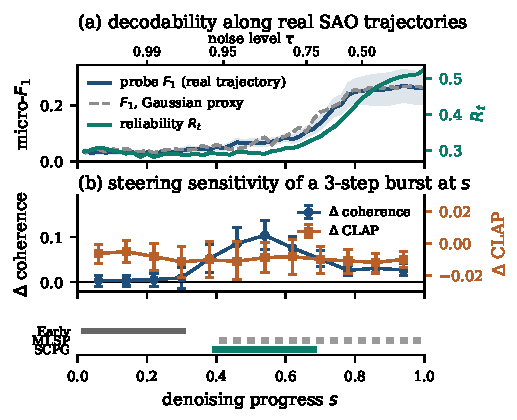
\includegraphics[width=\linewidth]{fig_trajectory.pdf}
\caption{(a) Probe reliability along 50 real SAO development trajectories (5 prompts $\times$ 10 seeds): micro-$F_1$ against pYIN labels of the generated audio, the target-free reliability $R_t$ of Eq.~\eqref{eq:rel}, and the Gaussian-noise proxy of~\cite{ye2026pitchclass} at matched noise level. (b) Interventional steering sensitivity: change in coherence and in CLAP from guidance at one position only (mean, 95\% CI, 50 paired development trials). Positions index the latent after the scheduler update; top axis: its noise level as the flow-time equivalent $t{=}\sigma/(1{+}\sigma)$, $\sigma$ the noise-to-signal rms ratio. Strip: steps of the Early, MLSP-fixed and SCPG schedules.}
\label{fig:traj}
\end{figure}

\subsection{Guidance window ablation and SCPG}
\label{sec:expB}
Table~\ref{tab:main} reports every schedule at the same budget of $K{=}15$ updates. Three findings stand out. First, placement is the dominant factor: at identical budget the early window barely improves over unguided SAO ($0.17$ vs $0.13$), the mid window more than triples it ($0.42$), and the late and MLSP windows fall in between. Second, the two calibrated schedules make the gap concrete. Because $F_1(t)$ increases monotonically, the top-$K$ steps of the decodability-calibrated ablation are exactly the late window (35--49), so its comparison with Late isolates $R$-scaling, which changes nothing there ($0.310$ vs $0.315$); SCPG selects steps 19--33 (18--32 at $\lambda{=}0.05$), i.e.\ it recovers the Mid window without a window sweep, and reaches \cohTopK\ against \cohMLSP\ for MLSP-fixed ($\pTopKvsMLSP$) and \cohMid\ for Mid ($\dTopKvsMid$, $\pTopKvsMid$); the contribution is the procedure that finds this window, not a schedule that beats it. Third, on SAO the control gain has no measurable quality cost. CLAP is preserved ($0.321$--$0.324$ for the SCPG variants vs $0.316$ for MLSP-fixed and $0.307$ unguided; no guided method differs significantly from MLSP-fixed) and the Fr\'echet distance to real piano is comparable ($0.75$--$0.76$ vs $0.79$; from 225 samples it is upward-biased and given for orientation only). The gain is not explained by reduced voicing (pYIN-voiced fraction $0.88$ under SCPG, $0.86$ MLSP-fixed, $0.84$ unguided), and coherence exceeds what the same audio would score if collapsed onto the melody's first pitch class ($0.445$ vs $0.255$), so the guidance follows the time-varying melody. pYIN is monophonic, so on polyphonic output the metric scores each frame's dominant pitch; chroma agreement is reported alongside it.

The advantage over MLSP-fixed holds for four of the five melodies and is within noise on the alternating arpeggio ($0.327$ vs $0.346$). The online variant, which thresholds each sample's own reliability, does not improve over MLSP-fixed ($0.351$ vs $0.363$, $p{=}0.53$): because $R_t$ tracks decodability, the threshold admits mostly late steps, which agrees with Sec.~\ref{sec:expC}, where decodability peaks later than steerability. $R$-scaling adds a small but consistent gain (\cohRAPG\ vs \cohTopK: $\dRvsTopK$, better in \winsRvsTopK\ non-tied trials, $\pRvsTopK$; vs Mid $\dRvsMid$, $\pRvsMid$), but its realised mean step on the test set is $\lamRealised$ rather than $0.05$, so this gain cannot be separated from a 15\% larger average step; about \placementShare\ of the improvement over MLSP-fixed comes from placement alone.

\begin{table}[t]
\centering\footnotesize
\caption{Test set (15 prompts $\times$ 5 melodies $\times$ 3 seeds), all guided methods with $K{=}15$ updates ($n{=}225$ per row); schedules are calibrated on the disjoint development set. Means; bootstrap 95\% CI half-widths are $\leq 0.035$ for coherence and $\leq 0.017$ for CLAP. $^{+}$/$^{-}$: coherence significantly higher/lower than MLSP-fixed ($p<0.05$, paired Wilcoxon, Holm over the nine comparisons). FAD is CLAP-embedding Fr\'echet distance to real piano (225 samples, upward-biased); \#u.: probe updates.}
\label{tab:main}
\setlength{\tabcolsep}{3.5pt}
\begin{tabular}{lccccc}
\toprule
Method & Coh.\ $\uparrow$ & Chroma $\uparrow$ & CLAP $\uparrow$ & FAD $\downarrow$ & \#u.\\
\midrule
SAO (unguided) & 0.126$^{-}$ & 0.22 & 0.307 & 0.82 & 0\\
Early (0--14) & 0.166$^{-}$ & 0.28 & 0.312 & 0.81 & 15\\
Mid (18--32) & 0.424$^{+}$ & 0.54 & 0.317 & 0.77 & 15\\
Late (35--49) & 0.315$^{-}$ & 0.46 & 0.311 & 0.81 & 15\\
Uniform & 0.283$^{-}$ & 0.41 & 0.314 & 0.79 & 15\\
MLSP-fixed (20--48) & 0.363 & 0.48 & 0.316 & 0.79 & 15\\
Top-$K$($F_1$) + $R$-scaling & 0.310$^{-}$ & 0.46 & 0.310 & 0.81 & 15\\
$R$-threshold (online) & 0.351 & 0.45 & 0.314 & 0.77 & 15.0\\
SCPG: Top-$K$($\Delta C$) & 0.434$^{+}$ & 0.55 & 0.321 & 0.76 & 15\\
SCPG + $R$-scaling & 0.445$^{+}$ & 0.56 & 0.324 & 0.75 & 15\\
\bottomrule
\end{tabular}

\end{table}

\subsection{Budget sweep}
\label{sec:expD}
Fig.~\ref{fig:budget} varies the number of guided steps, $K\in\{\budgetKs\}$, on a paired subset of the test set (10 prompts $\times$ 5 melodies, one seed) for the uniform schedule and for SCPG with constant $\lambda$, so that only the placement of the budget differs. The sensitivity-placed budget dominates at every $K$ (paired Wilcoxon $p<10^{-5}$): ten sensitivity-selected updates recover 95\% of the coherence of twenty-five uniformly spread ones (\cohTopKx\ vs \cohUniKxxv), and at $K{=}25$ coherence reaches \cohTopKxxv\ against \cohUniKxxv\ without saturating, so the useful window is wider than 15 steps and the marginal profile is not simply additive. CLAP stays inside its confidence band at every budget. The sweep is single-seed and an efficiency analysis, not the primary comparison; its CLAP level differs from Table~\ref{tab:main} because the subset's prompts score higher for every method.

\begin{figure}[t]
\centering
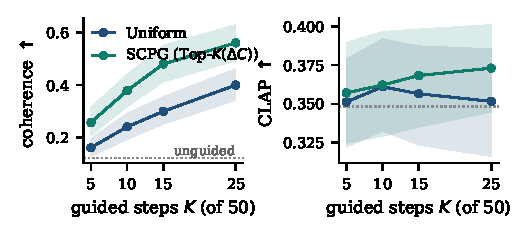
\includegraphics[width=\linewidth]{fig_budget.pdf}
\caption{Budget sweep on a paired 50-trial subset: coherence (left) and CLAP (right) against the number of guided steps, uniformly spread vs placed at the steps of highest steering sensitivity (mean, bootstrap 95\% CI). Dotted: unguided.}
\label{fig:budget}
\end{figure}

\subsection{Transfer to Stable Audio 3}
\label{sec:sa3}
To test whether the gap is specific to SAO 1.0, we repeated both analyses on the base checkpoint of Stable Audio 3 medium~\cite{evans2026stableaudio3}: a 1.4B-parameter flow-matching transformer (2.3B with autoencoder and text encoder) over 256-d latents at 10.8 frames/s, run for 50 Euler steps on its log-SNR-shifted schedule with CFG 7. A probe of the same architecture, trained on its latents with the recipe of~\cite{ye2026pitchclass}, reaches held-out micro-$F_1$ 0.59 (0.66 on SAO). The released checkpoints are post-trained with ARC~\cite{novack2025arc} for 8-step sampling, leaving a schedule only eight positions, so we analyse the base model. Fig.~\ref{fig:sa3} shows the same picture with the window elsewhere: decodability reaches 95\% of its maximum only at \saThreePeakF\ of denoising, tracked by $R_t$ (Pearson \saThreeCorrRF), whereas a burst is most effective early---sensitivity is flat within its CI at $\Delta C\approx\saThreeDCearly$ over the first 40\% of steps, which the shifted schedule keeps at noise level $t\ge0.95$ where the probe is at chance, and falls to \saThreeDClate\ in the last 20\%, where the probe is most accurate. In noise-level terms the two windows are adjacent rather than opposite. SAO's steps 18--32 span $\sigma\approx\sigmaAtEighteen\to\sigmaAtThirtyTwo$ ($t\approx\tAtEighteen\to\tAtThirtyTwo$) while SA3's plateau is $t\ge0.95$; what differs is that the near-pure-noise steps ($t>0.98$), inert on SAO, are effective on SA3. That a burst helps where the probe cannot yet read the latent is consistent with Sec.~\ref{sec:expC}: the gradient pushes along the directions the probe associates with the target pitch classes, and at high noise the sampler turns that push into structure.\RANDNOTESAThree\ Calibration selects steps \saThreeRAPGsteps; the plateau is flat, so any 15 steps inside it are near-equivalent, and the early window of~\cite{novack2026latch} (0--14) is one such choice. On 50 paired test trials (10 held-out prompts $\times$ 5 melodies, one seed) at $K{=}15$, SCPG reaches coherence \saThreeCohTopK\ (unguided \saThreeCohSAO) against \saThreeCohMLSP\ for the window of~\cite{ye2026pitchclass} (paired Wilcoxon $p{<}10^{-4}$) and \saThreeCohLate\ for the late window; the early window of~\cite{novack2026latch}, which barely moves pitch-class content on SAO at this step size, is within the CI of the calibrated schedule here (\saThreeCohEarly). Unlike on SAO, the gain is not free. CLAP falls from \saThreeClapSAO\ to \saThreeClapTopK\ under SCPG (Holm $p{<}0.01$), and every guided window except that of~\cite{ye2026pitchclass} (\saThreeClapMLSP, n.s.) shows a similar drop; FAD is not evaluated on SA3. Neither fixed window transfers between the two models, whereas the burst sweep finds the right window in both.

\begin{figure}[t]
\centering
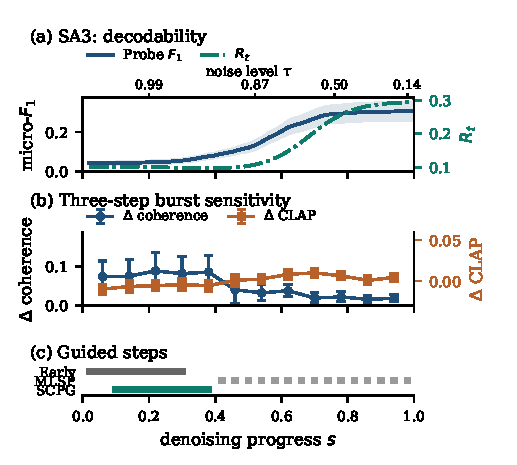
\includegraphics[width=\linewidth]{fig_sa3.pdf}
\caption{The same analysis on Stable Audio 3 medium (base, 50 steps): (a) probe micro-$F_1$ and reliability $R_t$ along 50 real development trajectories; (b) change in coherence and in CLAP from a 3-step burst at one position (mean, 95\% CI, 50 paired development trials). The top axis gives the sampler's noise level $t$ at each position.}
\label{fig:sa3}
\end{figure}


\section{Discussion and conclusion}
\label{sec:discussion}
What a probe can read from a latent and what a gradient step can \emph{write} into the output belong to different stages of denoising: readability grows until the latent is almost clean, but a nudge changes the music where coarse structure is still being decided. A schedule tuned to decodability spends its budget too late; tuning it to measured steering sensitivity recovers the best fixed window without a window sweep and at no inference cost. Image diffusion shows the same pattern: coarse content is decided at high noise~\cite{choi2022p2} and intermediate latents are the most editable~\cite{kwon2023hspace}. Reliability remains useful as a diagnostic and as a strength modulator, but it should not choose the placement. The sweet spot differs between models: on Stable Audio 3 it sits at the noisy start of the trajectory, so a window tuned on one model is wrong on the other, whereas one burst sweep on a few development prompts finds it in both. Limits: pitch-class control, guidance on $\z_t$, 50-step samplers, unvalidated quality proxies.

\vfill\pagebreak
\bibliographystyle{IEEEbib}
\bibliography{refs}

\section{Compliance with ethical standards}
This study used only publicly available pretrained models (Stable Audio Open 1.0 and the Stable Audio 3 medium base checkpoint, both under the Stability AI Community License) and datasets (MAESTRO), and generated synthetic audio; it involved no human or animal subjects, and no ethical approval was required.

\end{document}
